\documentclass[12pt,,]{report}
\usepackage{lmodern}
\usepackage{amssymb,amsmath}
\usepackage{ifxetex,ifluatex}
\usepackage{fixltx2e} % provides \textsubscript
\ifnum 0\ifxetex 1\fi\ifluatex 1\fi=0 % if pdftex
  \usepackage[T1]{fontenc}
  \usepackage[utf8]{inputenc}
\else % if luatex or xelatex
  \ifxetex
    \usepackage{mathspec}
  \else
    \usepackage{fontspec}
  \fi
  \defaultfontfeatures{Ligatures=TeX,Scale=MatchLowercase}

    \usepackage{xeCJK}
    % 中文自動換行
    \XeTeXlinebreaklocale "zh"
    % 文字的彈性間距
    \XeTeXlinebreakskip = 0pt plus 1pt
    \newfontlanguage{Chinese}{CHN}
    % 章次20級,節次16級,小節次以下14級,本文12級字
    \def\LARGE{\fontsize{20}{30}\selectfont}%章次
    \def\Large{\fontsize{16}{24}\selectfont}%節次
    \def\large{\fontsize{14}{21}\selectfont}%小節次
    \usepackage{indentfirst}
    \usepackage{CJKnumb}
    \renewcommand{\figurename}{圖}
    \renewcommand{\thefigure}{{\arabic{chapter}}.\arabic{figure}}
    \renewcommand{\tablename}{表}
    \renewcommand{\thetable}{{\arabic{chapter}}.\arabic{table}}
    %重製章節
    \renewcommand{\chaptername}{}
    \renewcommand{\thechapter}{第\CJKnumber{\arabic{chapter}}章}
    \renewcommand{\thesection}{{\arabic{chapter}}.\arabic{section}}
    \renewcommand{\thesubsection}{{\arabic{chapter}}.{\arabic{section}}.\arabic{subsection}}
    %設定行距與中英文字型
    \linespread{1}\selectfont
    \setCJKmainfont{SimSun}
    \setmainfont{Times New Roman}
    \setromanfont{Times New Roman}
    \setmonofont{Times New Roman}
    %重製章節標籤
    \usepackage{titlesec}
    \titleformat{\chapter}[block]{\LARGE\centering}{\thechapter}{0.5em}{}
    \titleformat{\section}[block]{\Large}{\thesection}{0.5em}{}
    \titleformat{\subsection}[block]{\large}{\thesubsection}{0.5em}{}
    % 重製目錄
    \usepackage{titletoc}
    \titlespacing{\chapter}{0pt}{*0}{*2}
    \titlespacing{\section}{0pt}{*1}{*1}
    \titlespacing{\subsection}{0pt}{*1}{*1}
    \titlespacing{\subsubsection}{0pt}{*1}{*1}
    \titlecontents{chapter}[0em]{}{\contentspush{\thecontentslabel}\hspace*{1em}}{}{\titlerule*[0.7pc]{.}\contentspage}
\fi
% use upquote if available, for straight quotes in verbatim environments
\IfFileExists{upquote.sty}{\usepackage{upquote}}{}
% use microtype if available
\IfFileExists{microtype.sty}{
\usepackage{microtype}
\UseMicrotypeSet[protrusion]{basicmath} % disable protrusion for tt fonts
}{}
\usepackage[margin=1in]{geometry}
\usepackage[unicode=true]{hyperref}
\hypersetup{
            pdfauthor={設計一乙 40623219 XXX; 設計一乙 40623220 蔡崇廷; 設計一乙 40623221 蔡和勳; 設計一乙 40623228 陳永錩; 設計一乙 40623229 陳宥安; 設計一乙 40623230 陳柏亦},
            pdfborder={0 0 0},
            breaklinks=true}
\urlstyle{same}  % don't use monospace font for urls
\ifnum 0\ifxetex 1\fi\ifluatex 1\fi=0 % if pdftex
  \usepackage[shorthands=off,main=]{babel}
\else
  \usepackage{polyglossia}
  \setmainlanguage[]{}
\fi
\usepackage{graphicx,grffile}
\makeatletter
\def\maxwidth{\ifdim\Gin@nat@width>\linewidth\linewidth\else\Gin@nat@width\fi}
\def\maxheight{\ifdim\Gin@nat@height>\textheight\textheight\else\Gin@nat@height\fi}
\makeatother
% Scale images if necessary, so that they will not overflow the page
% margins by default, and it is still possible to overwrite the defaults
% using explicit options in \includegraphics[width, height, ...]{}
\setkeys{Gin}{width=\maxwidth,height=\maxheight,keepaspectratio}
\IfFileExists{parskip.sty}{%
\usepackage{parskip}
}{% else
\setlength{\parindent}{0pt}
\setlength{\parskip}{6pt plus 2pt minus 1pt}
}
\setlength{\emergencystretch}{3em}  % prevent overfull lines
\providecommand{\tightlist}{%
  \setlength{\itemsep}{0pt}\setlength{\parskip}{0pt}}
\setcounter{secnumdepth}{5}
% Redefines (sub)paragraphs to behave more like sections
\ifx\paragraph\undefined\else
\let\oldparagraph\paragraph
\renewcommand{\paragraph}[1]{\oldparagraph{#1}\mbox{}}
\fi
\ifx\subparagraph\undefined\else
\let\oldsubparagraph\subparagraph
\renewcommand{\subparagraph}[1]{\oldsubparagraph{#1}\mbox{}}
\fi

% set default figure placement to htbp
\makeatletter
\def\fps@figure{htbp}
\makeatother


\begin{document}
%Cover Start
\begin{titlepage}
\vspace{1cm}
\begin{center}
\fontsize{36}{54}\selectfont{
    國立虎尾科技大學\par
}
\fontsize{28}{42}\selectfont{機械設計工程系\par}
\fontsize{24}{36}\selectfont{計算機程式 bg5 期末報告\par}
\vspace{1.5cm}
\fontsize{20}{30}\selectfont{
    PyQt5 事件導向計算器\par
    PyQt5 Event-Driven Calculator Project\par
}
\vspace{\fill}
\fontsize{18}{27}\selectfont{
    學生:\par
    設計一乙 40623219 XXX \par 設計一乙 40623220 蔡崇廷 \par 設計一乙 40623221 蔡和勳 \par 設計一乙 40623228 陳永錩 \par 設計一乙 40623229 陳宥安 \par 設計一乙 40623230 陳柏亦 \par
    指導教授:嚴家銘\par
}
\vspace{1.5cm}
\fontsize{16}{24}\selectfont{2017.12.25\par}
\end{center}
\vspace{1cm}
\end{titlepage}

\newcommand\frontmatter{
    \cleardoublepage
    \pagenumbering{roman}
}

\newcommand\mainmatter{
    \cleardoublepage
    \pagenumbering{arabic}
}

\newcommand\backmatter{
    \if@openright
        \cleardoublepage
    \else
        \clearpage
    \fi
}

%Document start

% Set page number to arabic i ii...
\frontmatter
\renewcommand{\abstractname}{\LARGE \center 摘要}
\chapter*{摘要}
\addcontentsline{toc}{chapter}{摘要}
\fontsize{14}{21}\selectfont{這裡是摘要內容。A pipe character, followed by an indented block of text
is treated as a literal block, in which newlines are preserved
throughout the block, including the final newline.

\begin{itemize}
\tightlist
\item
  以 YAML 的方式插入。
\item
  The `+' indicator says to keep newlines at the end of text blocks.
\item
  使用 Markdown 語法。
\item
  前面使用加號
\end{itemize}

本研究的重點在於 \ldots{}}


\begingroup
    \renewcommand{\contentsname}{\center 目錄 \addcontentsline{toc}{chapter}{目錄}}
    \renewcommand{\numberline}[1]{~#1\hspace*{1em}}
        \setcounter{tocdepth}{2}
    \tableofcontents
    \newcommand{\lotlabel}{表}
    \renewcommand{\listtablename}{\center 表目錄 \addcontentsline{toc}{chapter}{表目錄}}
    \renewcommand{\numberline}[1]{\lotlabel~#1\hspace*{1em}}
    \listoftables
    \newcommand{\loflabel}{圖}
    \renewcommand{\listfigurename}{\center 圖目錄 \addcontentsline{toc}{chapter}{圖目錄}}
    \renewcommand{\numberline}[1]{\loflabel~#1\hspace*{1em}}
    \listoffigures
\endgroup

% Start normal page number, 1 2 3
\mainmatter
\hypertarget{ux524dux8a00}{%
\chapter{前言}\label{ux524dux8a00}}

計算器程式期末報告前言

\hypertarget{ux53efux651cux7a0bux5f0fux7cfbux7d71ux4ecbux7d39}{%
\chapter{可攜程式系統介紹}\label{ux53efux651cux7a0bux5f0fux7cfbux7d71ux4ecbux7d39}}

\hypertarget{ux555fux52d5ux8207ux95dcux9589}{%
\section{啟動與關閉}\label{ux555fux52d5ux8207ux95dcux9589}}

\begin{figure}
\centering
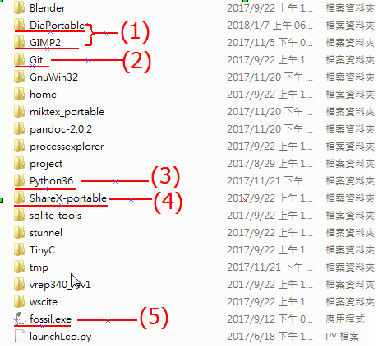
\includegraphics{./tex2pdf.5720/caf4a9154d74acc2785da5493d834ee1f5907b1f.png}
\caption{system-1\label{fig:格子}}
\end{figure}

可攜程式:因為在不同的電腦擁有的程式也會有所不同所以使用可攜程式的話可以方便在任何電腦執行自己熟悉的程式也可使用建立自己習慣的開發環境

(1)GIMP2-可以做修剪圖片或是裁切圖片

DiaPortable-可繪製圖形幫助註解圖片

(2)GitHub-SCM(組態管理系統)的一種 ,
特點多人協同,gh-pages,公開(不公開要花錢)

(3)Python36-在不同電腦都可以進行Python的程式開發

(4)ShareX-可截取螢幕畫面 , 與錄製影片

(5)Fossil-SCM(組態管理系統)的一種 , 特點Totally control
完全可以自己控制伺服到客戶端

\hypertarget{ux555fux52d5ux8207ux95dcux95892}{%
\section{啟動與關閉2}\label{ux555fux52d5ux8207ux95dcux95892}}

\begin{figure}
\centering
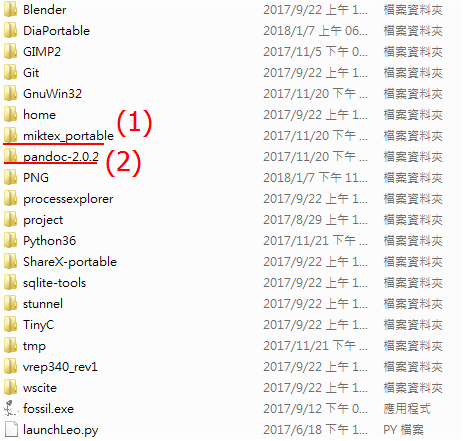
\includegraphics{./tex2pdf.5720/4cb54a5c1c7300c7281ffa6c61f663abf48448ba.png}
\caption{system-2\label{fig:格子}}
\end{figure}

(1)miktex\_portable-包含了TeX及其相關程式 ,
這些工具是以TeX/LaTeX所構成的

(2)pandoc-2.0.2-以命令列形式實現與用戶的互動,可支援多種作業系統

可攜程式系統介紹

\hypertarget{calculator-ux7a0bux5f0f}{%
\chapter{Calculator 程式}\label{calculator-ux7a0bux5f0f}}

Calculator 程式細部說明

\hypertarget{ux5efaux7acbux5c0dux8a71ux6846}{%
\section{建立對話框}\label{ux5efaux7acbux5c0dux8a71ux6846}}

step1

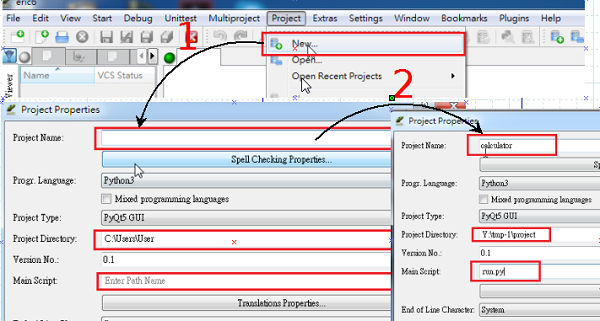
\includegraphics{./tex2pdf.5720/c57e7a0fedaa64e113d47539b62000be4e322d2a.png}
step2

\begin{figure}
\centering
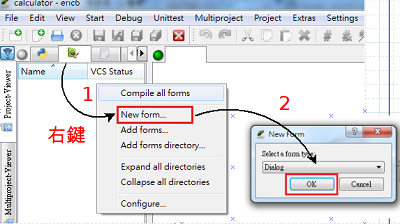
\includegraphics{./tex2pdf.5720/c25bd9e4292b8e505371b402e65eff0381a50874.png}
\caption{newform\label{fig:新建}}
\end{figure}

step3

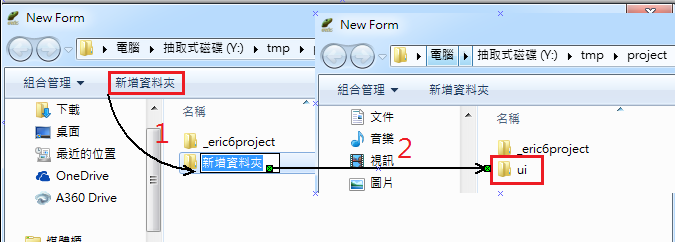
\includegraphics{./tex2pdf.5720/b71e9cd709a8d6470e96d63a7b4be8086a2eafc2.png}
step4

\begin{figure}
\centering
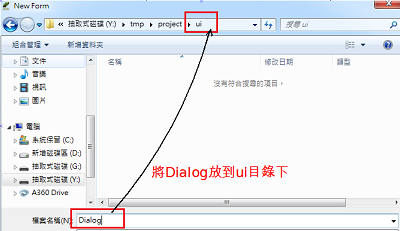
\includegraphics{./tex2pdf.5720/b6c557891824123971bab6160b93017a946ced9a.png}
\caption{Dialog into ui\label{fig:放入}}
\end{figure}

step5

\begin{figure}
\centering
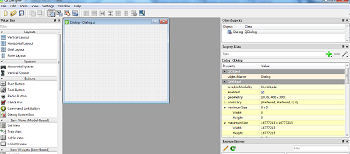
\includegraphics{./tex2pdf.5720/abab883aad37fc9d5d8430daf240ac70fd7b79ca.png}
\caption{qtdesigner\label{fig:對話框}}
\end{figure}

\hypertarget{ux5efaux7acbux6309ux9215}{%
\section{建立按鈕}\label{ux5efaux7acbux6309ux9215}}

step1

\begin{figure}
\centering
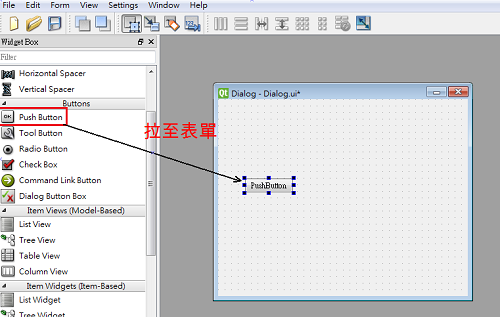
\includegraphics{./tex2pdf.5720/c6dc00a1f7430efee507473486a08a0400a99cfe.png}
\caption{button\label{fig:格子}}
\end{figure}

step2

\begin{figure}
\centering
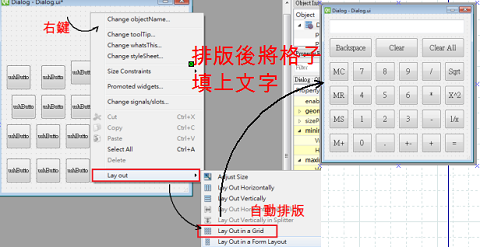
\includegraphics{./tex2pdf.5720/5adf72ef7cc9374dcc293eda6ce7834a69361a58.png}
\caption{grid\label{fig:排版}}
\end{figure}

以上是由Qtdesigner製作

Qtdesigner詳細請查閱第五章

\hypertarget{ux5efaux7acbux7a0bux5f0fux78bc}{%
\section{建立程式碼}\label{ux5efaux7acbux7a0bux5f0fux78bc}}

\textbf{40623220}

\begin{itemize}
\item
\end{itemize}

乘除

\begin{figure}
\centering
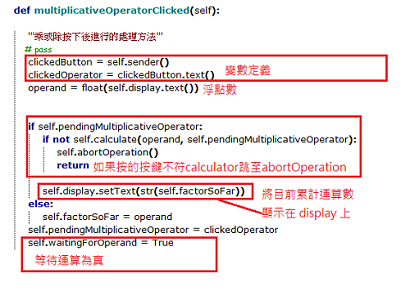
\includegraphics{./tex2pdf.5720/0b1409658ad8bf80f66fd4636009ff033b21fa47.png}
\caption{mult\label{fig:乘除}}
\end{figure}

變號

\begin{figure}
\centering
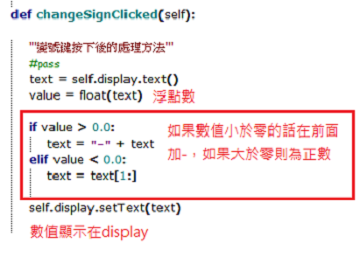
\includegraphics{./tex2pdf.5720/c2b33670cf8de1ed5272a762b63b229061af4784.png}
\caption{change\label{fig:變號}}
\end{figure}

計算

\begin{figure}
\centering
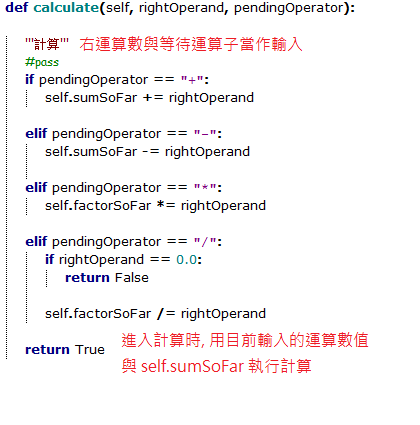
\includegraphics{./tex2pdf.5720/90b5c4696f030346adac82021ab087edf71bb49b.png}
\caption{calculator\label{fig:計算}}
\end{figure}

中斷運算

\begin{figure}
\centering
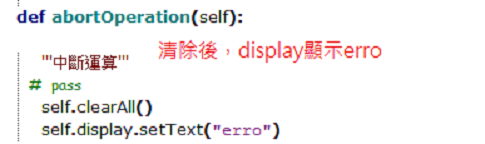
\includegraphics{./tex2pdf.5720/5df65b89e38b47ae806d7c8dc7fd862b3c52776e.png}
\caption{abo\label{fig:中斷運算}}
\end{figure}

\textbf{40623221}

\begin{verbatim}
def unaryOperatorClicked(self):
\end{verbatim}

\#40623221 '`'單一運算元按下後處理方法''' \#pass clickedButton =
self.sender() clickedOperator = clickedButton.text() operand =
float(self.display.text())

\begin{verbatim}
    if clickedOperator == "Sqrt":
        if operand < 0.0:
            self.abortOperation()
            return

        result = math.sqrt(operand)
    elif clickedOperator == "X^2":
        result = math.pow(operand, 2.0)
    elif clickedOperator == "1/x":
        if operand == 0.0:
            self.abortOperation()
            return

        result = 1.0 / operand

    self.display.setText(str(result))
    self.waitingForOperand = True
    
    說明:按下1/x若分母為0則需中斷運算,若按下Sqrt且數字小於0也是中斷運算,
    按下X^2若數字為2則需運算2的平方..
    
    def pointClicked(self):
\end{verbatim}

\#40623221 '`'小數點按下.後的處理方法''`\#pass if
self.waitingForOperand: self.display.setText('0')

\begin{verbatim}
    if "." not in self.display.text():
        self.display.setText(self.display.text() + ".")

    self.waitingForOperand = False
    
    說明:若出現display,且在數字0後面沒出現小數點則將小數點顯示出來..
    
     def clearAll(self):
\end{verbatim}

\#40623221 '`'全部清除鍵按下後的處理方法''`\#pass self.sumSoFar = 0.0
self.factorSoFar = 0.0 self.pendingAdditiveOperator
='`self.pendingMultiplicativeOperator ='`self.display.setText('0')
self.waitingForOperand = True

\begin{verbatim}
    說明:按下clearall則把全部運算停止並將全部情除最後出現0
    
\end{verbatim}

\textbf{40623228}

數字邏輯

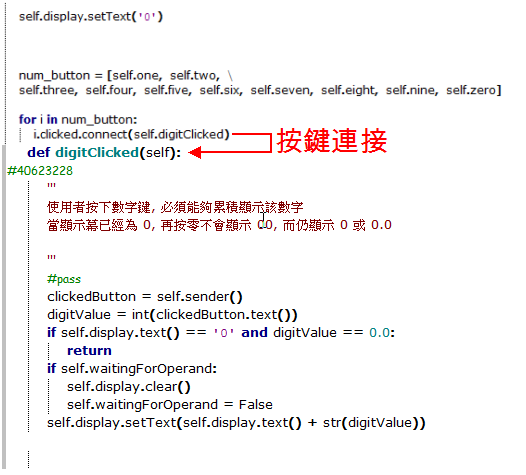
\includegraphics{./tex2pdf.5720/c2fc0212c0c1eb6e23fcceb61c5c33768d3624f8.png}
加減邏輯

\begin{figure}
\centering
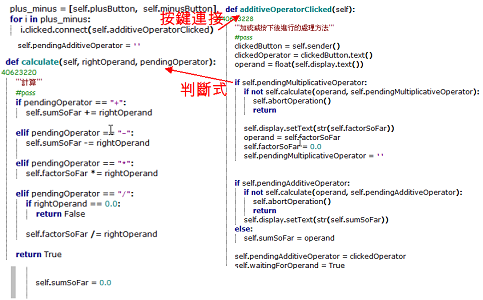
\includegraphics{./tex2pdf.5720/f8e1adba5ca9ef4f984bd3136a27e2a06fe35bd7.png}
\caption{additiveOperatorCliked\label{fig:additiveOperatorCliked}}
\end{figure}

等號邏輯

\begin{figure}
\centering
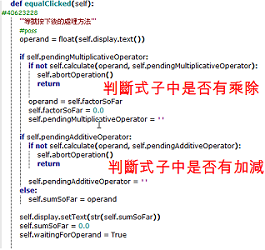
\includegraphics{./tex2pdf.5720/94c8a4b17bc1fa9edb4acf49cbd39f03992fc57d.png}
\caption{equalClicked\label{fig:equalClicked}}
\end{figure}

\textbf{40623229} '`'回復鍵按下的處理方法''' \#pass if
self.waitingForOperand: return

\begin{verbatim}
     text = self.display.text()[:-1]
     if not text:
         text = '0'
         self.waitingForOperand = True

     self.display.setText(text)
     if self.waitingForOperand:
         return
 def clear(self):
  
   '''清除鍵按下後的處理方法'''
     #pass
     if self.waitingForOperand:
         return

     self.display.setText('0')
     
     self.waitingForOperand = True
\end{verbatim}

\textbf{40623230}

\begin{verbatim}
def clearMemory(self):
\end{verbatim}

\#40623230 '`'清除記憶體鍵按下後的處理方法''' \#pass self.sumInMemory =
0.0

\begin{verbatim}
    說明:按下MC鍵後將記憶的數字變為0
    
def readMemory(self):
\end{verbatim}

\#40623230 '`'讀取記憶體鍵按下後的處理方法''' \#pass
self.display.setText(str(self.sumInMemory)) self.waitingForOperand =
True

\begin{verbatim}
    說明:按下MR鍵後把記憶的數字顯示出來
    
def setMemory(self):
\end{verbatim}

\#40623230 '`'設定記憶體鍵按下後的處理方法''' \#pass self.equalClicked()
self.sumInMemory = float(self.display.text())

\begin{verbatim}
    說明:按下MS鍵後會把當前的數字取代記憶的數字
    
def addToMemory(self):
\end{verbatim}

\#40623230 '`'放到記憶體鍵按下後的處理方法''' \#pass self.equalClicked()
self.sumInMemory += float(self.display.text())

\begin{verbatim}
    說明:按下M+鍵會把當前數字與記憶的數字相加後並記憶
\end{verbatim}

\hypertarget{python-ux7a0bux5f0fux8a9eux6cd5}{%
\chapter{Python 程式語法}\label{python-ux7a0bux5f0fux8a9eux6cd5}}

Python 程式語法

\hypertarget{ux8b8aux6578ux547dux540d}{%
\section{變數命名}\label{ux8b8aux6578ux547dux540d}}

Python3 變數命名規則與關鍵字

一、Python 英文變數命名規格

1.變數必須以英文字母大寫或小寫或底線開頭

2.變數其餘字元可以是英文大小寫字母, 數字或底線

3.變數區分英文大小寫

4.變數不限字元長度

5.不可使用關鍵字當作變數名稱

二、Python3 的程式關鍵字, 使用者命名變數時, 必須避開下列保留字.

1.Python keywords: {[}`False', `None', `True', `and', `as', `assert',
`break', `class', `continue', `def', `del', `elif', `else', `except',
`finally', `for', `from', `global', `if', `import', `in', `is',
`lambda', `nonlocal', `not', `or', `pass', `raise', `return', `try',
`while', `with', `yield'{]}

2.選擇好的變數名稱:

使用有意義且適當長度的變數名稱, 例如: 使用 length 代表長度,
不要單獨使用 l 或 L, 也不要使用 this\_is\_the\_length
程式前後變數命名方式盡量一致, 例如: 使用 rect\_length 或 RectLength
用底線開頭的變數通常具有特殊意義

計算機中的迴圈

\begin{figure}
\centering
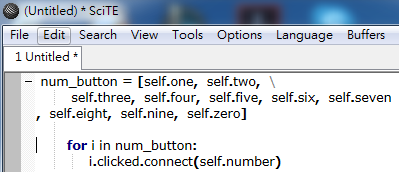
\includegraphics{./tex2pdf.5720/106aca04d9385e9a9d229e278f54864f570d52d5.png}
\caption{for\label{fig:迴圈}}
\end{figure}

\hypertarget{print-ux51fdux5f0f}{%
\section{print 函式}\label{print-ux51fdux5f0f}}

\hypertarget{ux91cdux8907ux8ff4ux5708}{%
\section{重複迴圈}\label{ux91cdux8907ux8ff4ux5708}}

\hypertarget{ux5224ux65b7ux5f0f}{%
\section{判斷式}\label{ux5224ux65b7ux5f0f}}

if 判斷式1:

\begin{verbatim}
要處理的指令1
\end{verbatim}

elif 判斷式2:

\begin{verbatim}
要處理的指令2
\end{verbatim}

else: 要處理的指令3

注意事項

1.每個判斷式的結束要加:

2.要處理的指令不可以用\{\}括起來

3.最後的else可以不用加

\hypertarget{ux6578ux5217}{%
\section{數列}\label{ux6578ux5217}}

python的數列是一個{[} {]}

{[} {]}是容器中能放容器也能放物件和字串

容器例如:list、set、dict、tuple

計算機中的數列

\begin{figure}
\centering
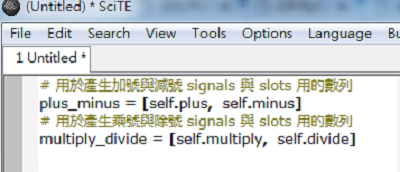
\includegraphics{./tex2pdf.5720/f4203eb0a9255f7eac1ae2abb9edd89f72c6dfcc.png}
\caption{s\label{fig:數列}}
\end{figure}

\hypertarget{pyqt5-ux7c21ux4ecb}{%
\chapter{PyQt5 簡介}\label{pyqt5-ux7c21ux4ecb}}

說明 PyQt5 基本架構與程式開發流程

\hypertarget{pyqt5-ux67b6ux69cb}{%
\section{PyQt5 架構}\label{pyqt5-ux67b6ux69cb}}

PyQt5-GUI frame work , 圖形使用者介面軟體框架 ,可以快速製做GUI界面程式 ,
是由一系列Python组成。超過620個類,6000和函數和方法

Qt5原本是C++語法 之後用Python製作而成PyQt

Qt採用了signal和slot的概念來處理GUI程式中的用戶事件。
PyQt同樣支援這種方法。
任何Python類型都可以定義signal和slot,並與GUI控制項的signal和slot相連線。

\hypertarget{ux5fc3ux5f97}{%
\chapter{心得}\label{ux5fc3ux5f97}}

期末報告心得

\hypertarget{fossil-scm}{%
\section{Fossil SCM}\label{fossil-scm}}

40623220蔡崇廷

學習到如何用指令維護倉儲還有wiki和timeline使用

40623221 蔡和勳

fossil 是比較簡單的一些指令所以一開始我們已fossil
當基礎練習了半學期將指令弄熟了其實跟 github 的指令是大同小異

40623228 陳永錩 Fossil使用起來比之前用雲端軟體的效率及感覺
有很大的不一樣以版次來說能夠在每次都能做成一種版次就比雲端更可以處存自己設計的東西

40623229 陳宥安
剛開始第一次接觸fossil完完全全不知道在搞啥也不知道做甚麼用的用在哪裡
摸了兩個禮拜才懂得一些皮毛而已,後來經過老師講解才得以將前後串起來

40623230陳柏亦 fossil學習到的近遠端的倉儲維護還有版次處理

\hypertarget{ux7db2ux8a8cux5fc3ux5f97}{%
\section{網誌心得}\label{ux7db2ux8a8cux5fc3ux5f97}}

40623220蔡崇廷

將自己每周的學習進度記錄在網誌上,能夠為自己的學習能夠有個回想

40623221 蔡和勳

將平常上課所學的指令及程式碼運用讓自己的網誌可以更新

40623228 陳永錩 在每次上課都做一次網誌想筆記一樣
有效的將遇到的問題及學過的東西記錄下來

網誌心得 40623229 陳宥安 將每個禮拜老師的上課內容上傳到自己的網誌

40623230 陳柏亦 可以將上課的內容記錄下來之後要尋找看便很容易

\hypertarget{github-ux5354ux540cux5009ux5132}{%
\section{Github 協同倉儲}\label{github-ux5354ux540cux5009ux5132}}

40623220 蔡崇廷 學到如何在 github 建立倉儲,
也學到如何與其他人協同做報告跟計算機的專題, 也 知道有衝突時該如何解決

40623221 蔡和勳
透過與組員一起寫計算機程式能更快解決問題,協同報告可以自動編排也很方便,不用再將文字檔拉來拉去

40623228 陳永錩
雖然說跟Fossil一樣是SCM的東西可是加上了多人協同就有很大的不能像是怎麼解決衝突等等

Github協同倉儲 40623229 陳宥安 方便的討論如何製作一個報告
不會因為不在同一個地方而無法討論 印證了天涯若比鄰這句話

40623230 陳柏亦
可以共同協同很方便,更新檔案只要上傳下載就好,不過更新時容易衝突,需要去解決

\hypertarget{ux5b78ux54e1ux5fc3ux5f97}{%
\section{學員心得}\label{ux5b78ux54e1ux5fc3ux5f97}}

40623220 蔡崇廷
從一開始的不知道這節課要幹嘛漸漸的進入狀況也能每周把自己的學習做個紀錄

40623221 蔡和勳 雖然程式碼很多很嚇人,
但是如果有看老師教學影片就可以很快進入狀況可以學很快,
自己在花點時間就可以將程式完成

40623228 陳永錩
在經過整學期的課程我覺得,程式會是必學的一項技能,有了程式的幫忙才可以有效率的完成設計上的事情

40623229 陳宥安
這16個禮拜一直處在懵懵懂懂的狀態下,不懂的地方還是很多,反覆了看了影片我相信總有一天會摸出個所以然,下學期希望也一直保持像這學期這樣的好狀態

40623230陳柏亦
剛開始完全不會到學期末,已經把這學期的都理解的差不多,比起開始已經不太討厭程式了

\hypertarget{ux8aaaux660eux5404ux5b78ux54e1ux4efbux52d9ux8207ux57f7ux884cux904eux7a0b}{%
\section{說明各學員任務與執行過程}\label{ux8aaaux660eux5404ux5b78ux54e1ux4efbux52d9ux8207ux57f7ux884cux904eux7a0b}}

說明各學員任務與執行過程

40623220 蔡崇廷
做計算機和報告不像前七周是自己做自己的而現在是必須與同學協同所以更需要
討論也必須更注意排版不然一定會亂掉

40623221 蔡和勳 組員所負責的計算機程式內容不一樣
若前面的按鈕和排版沒做好後面就沒辦法接下去做,還有按鈕名稱也很重要,
錯誤的話會沒辦法執行計畫

40623228 陳永錩 必須將流程已有條理的方式 逐步的完成不然很容易亂了手腳

40623229 陳宥安
裏頭的程式語言其實不是很懂,如何能將一整串的文字組在一塊,加上一些符號竟然能夠成為一台計算機,需要的是不停的動腦不停的失敗再試反覆的操作直到完成

40623230陳柏亦
自己的程序必須要做好,不然可能因為自己的部分有出錯,導致其他人無法完成,所以需要討論好,不然很容易出錯

\hypertarget{ux7d50ux8ad6}{%
\chapter{結論}\label{ux7d50ux8ad6}}

期末報告結論

結論與建議

透過這次的小組期末報告合作,大家學會了使用共同倉儲來協同,理解了許多的語法,在操作上很熟練很多,了解到分工時每一個地方都很重要,必須討論好,若是自己部分有錯誤,會影響到其他人,再進行作業時必須確保不會出錯,這樣才能完成期末報告。

\hypertarget{ux53c3ux8003ux6587ux737b}{%
\chapter{參考文獻}\label{ux53c3ux8003ux6587ux737b}}


\end{document}
